
\subsection{Mechanical structure}
The design of the robot is influenced by the LEGO\textregistered Mindstorms\textregistered EV3 set. While the original set has a movable base without a manipulator arm. It also does not incorporate the Dynamixel AX-12A Smart Servos used in the final design so the decision to redesign the robot with inspiration from the LEGO\textregistered EV3 design was made. By developing and designing a new platform it gave the possibility to adapt the dimensions and fastenings. It also gave experience in manufacturing methods such as 3D-printing and Laser cutting. The final design is shown in Fig. \ref{fig:concept_rendering}
Consisting of seven Dynamixel\textregistered AX-12A Smart Servos for actuation, two on the base for locomotion and four on the arm and one for the gripping tool the robot has seven degrees of freedom. The main advantage of using the AX-12As is the possibility of connecting them in series which enables parallel control of all the joints. Additionally with the built in sensors the motors return feedback of the joint angles, angular speed, current draw, temperature to name a few.  

\begin{figure}
    \centering
    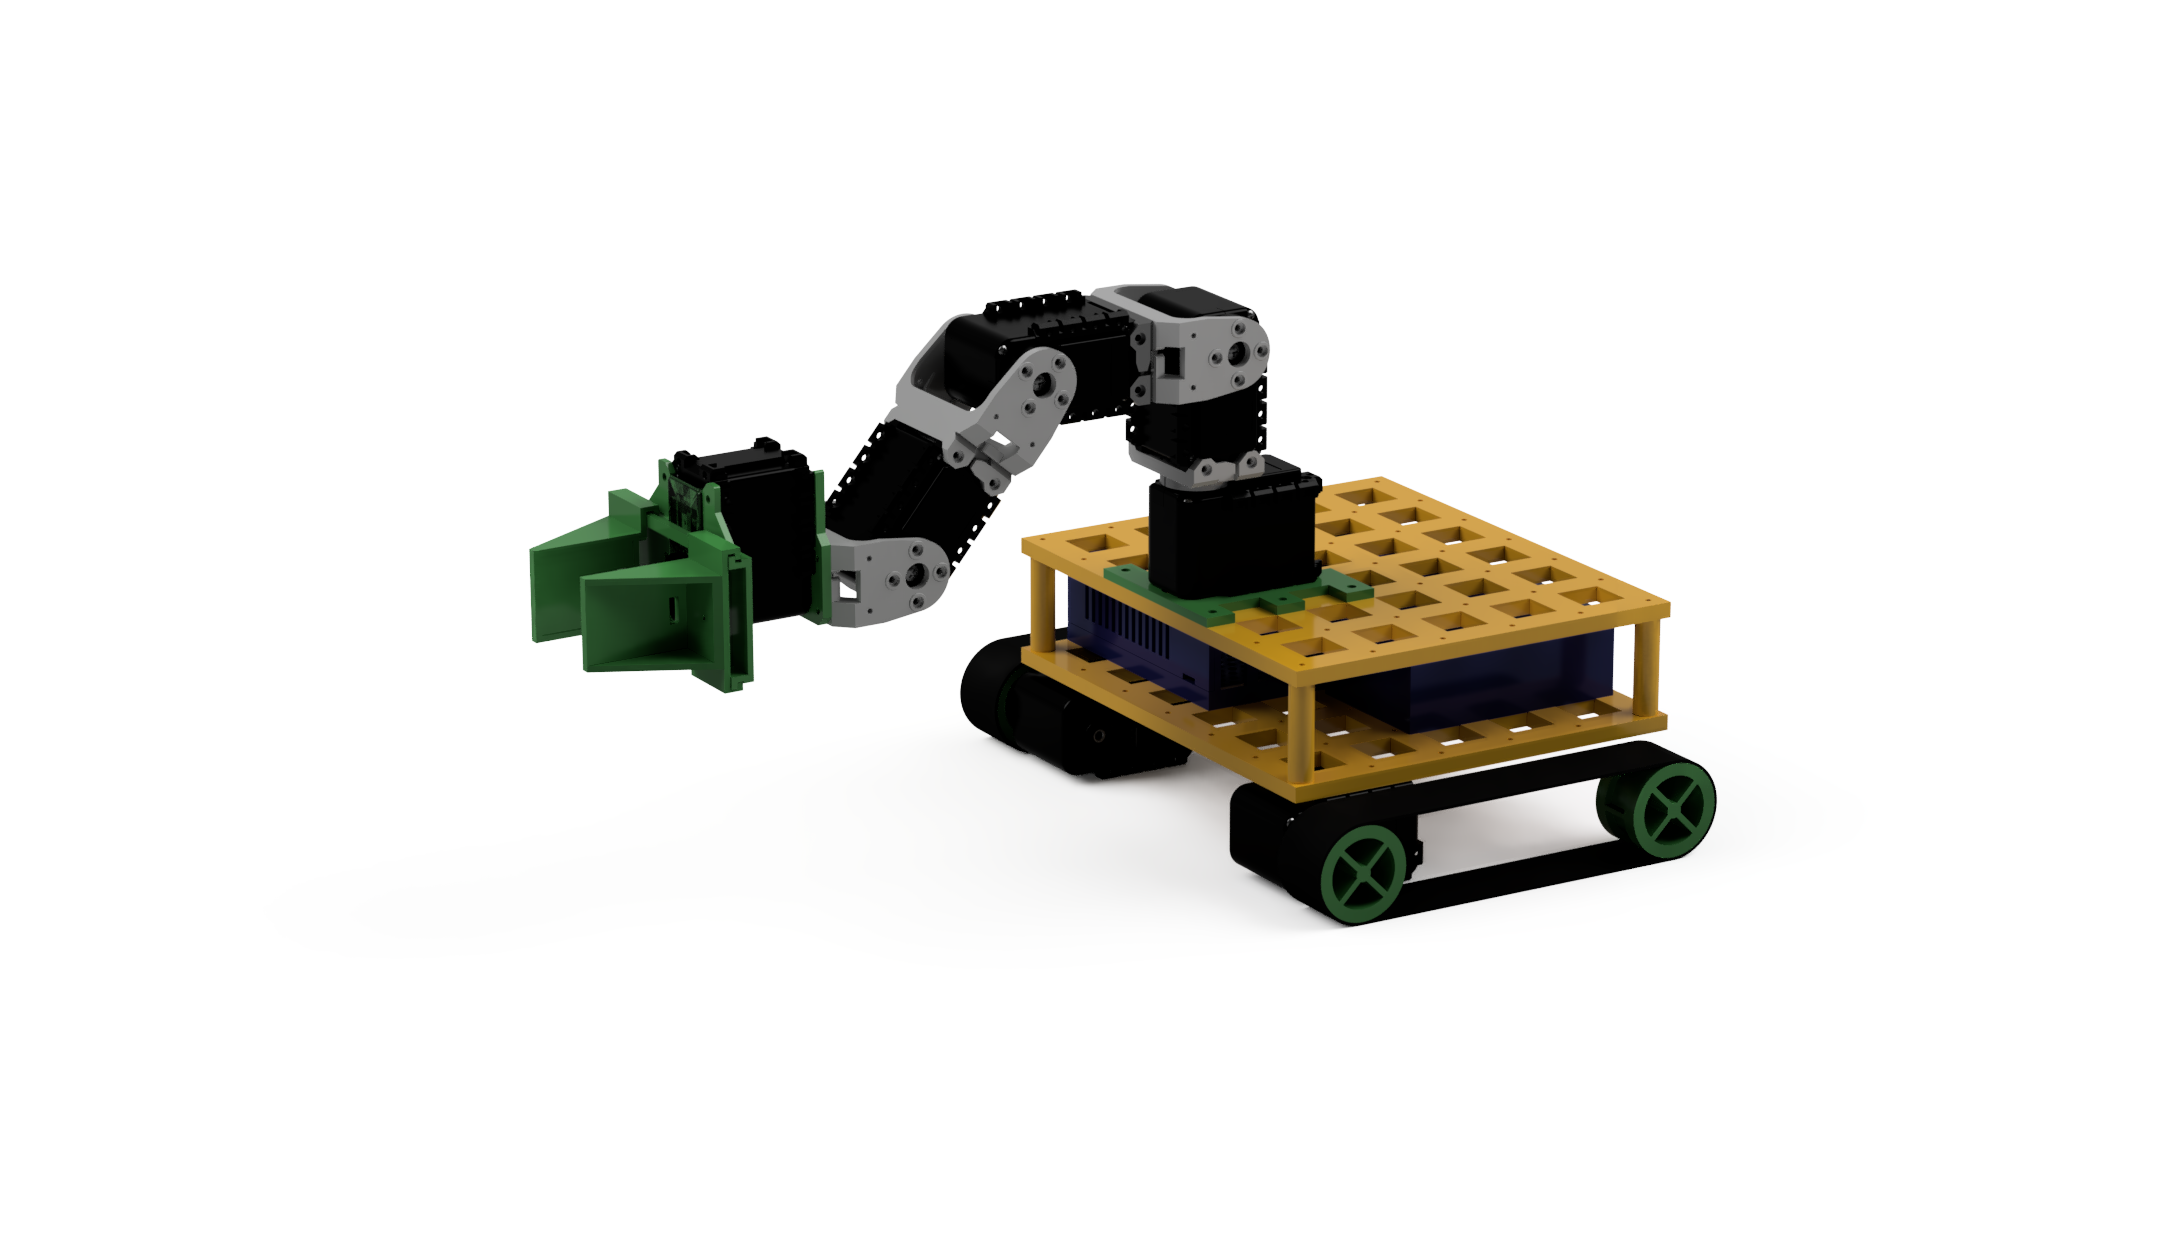
\includegraphics[width=0.7\columnwidth]{chapters/img/rendering.png}
    \caption{Rendering of concept design.}
    \label{fig:concept_rendering}
\end{figure}

\subsection{Electrical components}
While the mechanical components are those visible it's the underlying electrical components that make the big difference. The internals in the Dynamixel\textregistered AX-12A Smart Servo motors give feedback on the state of the motors, the 1000mAh LiPo battery supplies power to the motors and surrounding electronics. For the computations the NVIDIA\textregistered Jetson Nano is used as it runs Ubuntu natively which makes the implementation of the underlying Robotic Operating System (ROS) \cite{ros} faster. 
%\usetikzlibrary{shapes.geometric,arrows, positioning, fit}
\tikzstyle{computing} = [draw, rectangle, fill=white!50, rounded corners, node distance=3em, minimum height=3em]

\tikzstyle{io} = [rectangle, draw, trapezium right angle=110, rounded corners,
                  fill=red!20, node distance=5em, minimum height=2.9em]

\tikzstyle{calculate} = [diamond, draw, trapezium right angle=110, rounded corners,
                  fill=green!20, node distance=1.9cm, minimum height=2.9em]

\tikzstyle{hardware} = [rectangle, draw, trapezium right angle=110, rounded corners,
                  fill=blue!20, node distance=1.9cm, minimum height=2.9em]

\tikzstyle{external} = [rectangle, draw, trapezium right angle=110, rounded corners,
                  fill=gray!20, node distance=1.9cm, minimum height=2.9em]
\tikzstyle{line} = [draw, -latex']

\tikzstyle{function} = [rectangle, draw, fill=green!20, node distance=1.9cm, minimum height=2.9em]

    
    \begin{figure}
        \begin{center}
\resizebox{6.0cm}{!}{

\begin{tikzpicture}

    [align=center, auto]

        \node [computing] (lipo) {LiPo-battery};
        \node [computing, below= of lipo] (powerbank) {Power Pack};
        \node [computing, right= 5em of lipo] (motors) {Dynamixels};
        \node [computing, below= of motors] (nvidia) {NVIDIA};
        \coordinate [below= 1em of motors] (aux1);
        \coordinate [right= of aux1] (aux2);
        \node [computing, right= 5em of motors] (u2d2) {U2D2};
        \node [computing, below= of nvidia] (cameras) {Cameras};
        %\path [line] (nvidia)--(camera);

        \draw [-] (powerbank) -- node[midway, fill=white] {USB} (nvidia);
        \draw [-] (lipo) -- node[midway, fill=white] {2-wire} (motors);
        \draw [-] (motors) -- node[pos=0.5, fill=white] {3-wire} (u2d2);
        \draw [-] (nvidia) -| node[pos=0.25, fill=white] {USB} (u2d2);
        \draw [-] (nvidia) -- node[pos=0.5, fill=white] {CSI} (cameras);
    \end{tikzpicture}
    }
\end{center}
\caption{Diagram of electrical components}
\end{figure}


    %tikz/electrical_connections.tex

\subsection{Robotic Operating System}
Because the robot and the task consists of many different parts it is preferred to utilize an easy to use and well documented framework for internal communication on the robot. With its versatility and popularity within the research community this project makes use of the Robotic Operating System (ROS) as its underlying framework. 
ROS utilizes an internal TCP communication protocol where different parts can communicate and be synchronized which enables real-time performance. 
The rosgraph is shown in Fig. \ref{fig:rosgraph}. 

\begin{figure}
    \centering
    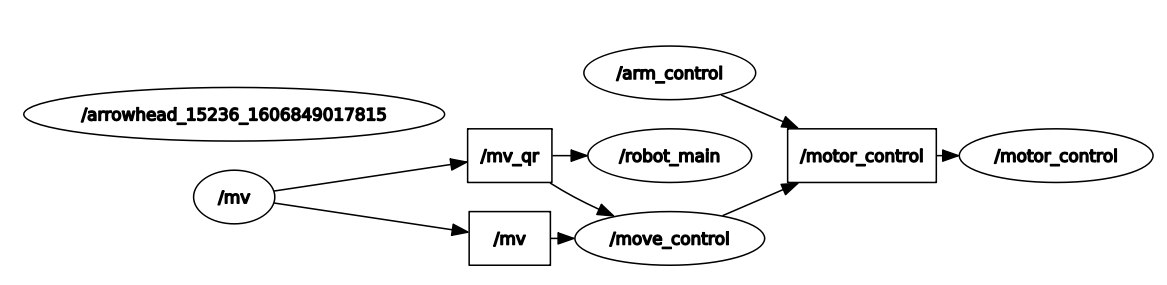
\includegraphics[width=0.7\columnwidth]{chapters/img/rosgraph.jpg}
    \caption{Rosgraph of the robot.}
    \label{fig:rosgraph}
\end{figure}



